\documentclass[aspectratio=169]{beamer}

% ------------------------------------------------------------
% Amurmaple theme (CTAN). Uses the BLUE option like your screenshot.
% ------------------------------------------------------------
\IfFileExists{beamerthemeAmurmaple.sty}{%
  \usetheme[amurmapleblue]{Amurmaple}
}{%
  \usetheme{Madrid}
  \usecolortheme{dolphin}
}


% ------------------------------------------------------------
% Packages
% ------------------------------------------------------------
\usepackage{amsmath}
\usepackage{amssymb}
\usepackage{physics}
\usepackage{graphicx}
\usepackage{tikz}
\usepackage{bm}
\usepackage{hyperref}
\usepackage{animate}
\usepackage[font=tiny]{caption}
\usepackage{microtype}
\setbeamertemplate{navigation symbols}{}

% ------------------------------------------------------------
% Convenience
%  - ./      : same folder as main.tex
%  - ../     : parent folder (YOUR Desktop, if project folder sits on Desktop)
%  - figures/: optional later
% ------------------------------------------------------------
\graphicspath{{./}{../}{figures/}}
\newcommand{\blanklines}[1]{\par\noindent\mbox{}\vspace{#1\baselineskip}\par}

% ------------------------------------------------------------
% UCD logo helper:
% Priority:
%  1) ucd-logo.png        (same folder as main.tex)
%  2) ../ucd-logo.png     (Desktop if main.tex is in Desktop/TMD-Analysis/)
%  3) figures/ucd-logo.png
%  4) fallback placeholder (no compile error)
% ------------------------------------------------------------
\newcommand{\UCDLogo}{%
  \IfFileExists{ucd-logo.png}{%
    \includegraphics[height=3cm]{ucd-logo.png}%
  }{%
    \IfFileExists{../ucd-logo.png}{%
      \includegraphics[height=1.4cm]{../ucd-logo.png}%
    }{%
      \IfFileExists{figures/ucd-logo.png}{%
        \includegraphics[height=1.4cm]{figures/ucd-logo.png}%
      }{%
        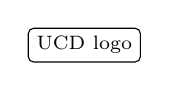
\begin{tikzpicture}[baseline]
          \node[draw, rounded corners=2pt, inner sep=3pt] {\scriptsize UCD logo};
        \end{tikzpicture}%
      }%
    }%
  }%
}

% --- Put logo on the title page (top-left) ---
\addtobeamertemplate{title page}{}{%
  \begin{tikzpicture}[remember picture,overlay]
    \node[anchor=north west, xshift=0.35cm, yshift=-0.25cm]
      at (current page.north west) {\UCDLogo};
  \end{tikzpicture}%
}

% ------------------------------------------------------------
% Fill-these-in fields (NO square-bracket placeholders)
% ------------------------------------------------------------
\title[Project Title]{A TMD-oriented analysis of pi+pi- pairs in e+e- collisions}
\subtitle{Herwig analysis / Theory}
\author{Shane Sweetman hello}
\institute{Project update meeting\\\\Student No: 22308373}
\date{}

\begin{document}

% ============================================================
% Title slide
% ============================================================
\begin{frame}[plain]
  \titlepage
\end{frame}

% ============================================================
% Slide 2: Aims / Question
% ============================================================
\section{Aims \& Research Question}
\begin{frame}{Quick Recap \& Aims}
  \begin{block}{Aim(s)}
    \vspace{-0.5em}
    \small
    \begin{itemize}
      \setlength{\itemsep}{0.35em}
      \setlength{\parskip}{0pt}
      \setlength{\parsep}{0pt}

      \item Fragmentation: how partons turn into hadrons, and why this needs non-perturbative modelling as the shower approaches $Q_0\sim 1~\mathrm{GeV}$. [6]

      \item Two main Monte-Carlo hadronisation approaches:
      \begin{itemize}
        \setlength{\itemsep}{0.25em}
        \setlength{\parskip}{0pt}
        \setlength{\parsep}{0pt}
        \item String hadronisation in \textsc{Pythia} (Lund). [5,4]
        \item Cluster hadronisation in \textsc{Herwig}. [7,9]
      \end{itemize}

      \item Reproduce the \textsc{Pythia} plots in \textsc{Herwig} and compare; differences can come from shower + hadronisation/tune. [4,9]

      \item Non-perturbative transverse-momentum modelling (intrinsic $k_T$ analogue) and its impact on $p_T$-type observables. [11,12,13]
    \end{itemize}
    \normalsize
    \vspace{-0.4em}
  \end{block}
\end{frame}

% ============================================================
% Slide 3: Fragmentation functions
% ============================================================
\section{Fragmentation functions}
\begin{frame}{Fragmentation functions: what matters}
  \begin{block}{}
    \vspace{-0.5em}
    \small
    \begin{itemize}
      \setlength{\itemsep}{0.35em}
      \setlength{\parskip}{0pt}
      \setlength{\parsep}{0pt}

      \item Fragmentation functions $D_i^h(z,Q)$: probability density for parton $i\to h$ with longitudinal momentum fraction $z$ at factorisation scale $Q$. [1,2]

      \item Collinear factorisation for inclusive $e^+e^-\to hX$:
      \[
        \frac{1}{\sigma_{\mathrm{tot}}}\frac{d\sigma(e^+e^- \to hX)}{dz}
        = \sum_i C_i(z,Q)\otimes D_i^h(z,Q),\qquad
        (C\otimes D)(z)\equiv \int_z^1 \frac{dy}{y}\, C(y,Q)\,D\!\left(\frac{z}{y},Q\right). [1,2]
      \]

      \item $D_i^h$ is non-perturbative but evolves with $Q$ (DGLAP); tuned using $e^+e^-$ data; treated as universal. [1,2,3]
    \end{itemize}
    \normalsize
    \vspace{-0.4em}
  \end{block}
\end{frame}

% ============================================================
% Slide 4: Lund / String picture (Pythia default)
% ============================================================
\section{Lund / String Hadronisation}
\begin{frame}{Lund / String picture (Pythia default)}
  \begin{block}{What the model is doing}
    \vspace{-0.5em}
    \small
    \begin{itemize}
      \setlength{\itemsep}{0.30em}
      \setlength{\parskip}{0pt}
      \setlength{\parsep}{0pt}

      \item In the Lund/string picture, showered coloured partons remain connected by colour flow; the colour field is modelled as a string with approximately constant tension. [5,4]

      \item As partons separate the string stores energy; it breaks by creating $q\bar q$ pairs, producing a chain of hadrons along the colour connection. [5]

      \item Longitudinal momentum sharing is described via a momentum fraction $z$ (fragmentation function form used internally by the model). [5,4]

      \item String breaking generates non-perturbative transverse momentum via back-to-back $p_T$ kicks for the created pair (width is a tunable knob). [4,12]
    \end{itemize}
    \normalsize
    \vspace{-0.4em}
  \end{block}
\end{frame}

% ============================================================
% Slide 5: Cluster picture (Herwig)
% ============================================================
\section{Cluster Hadronisation (Herwig)}
\begin{frame}{Cluster picture (Herwig default)}
  \begin{block}{Cluster hadronisation: what is happening}
    \vspace{-0.5em}
    \small
    \begin{itemize}
      \setlength{\itemsep}{0.35em}
      \setlength{\parskip}{0pt}
      \setlength{\parsep}{0pt}

      \item \textsc{Herwig} uses a cluster hadronisation model. [7,9]

      \item As the shower reaches the low-$Q$ cutoff, preconfinement implies colour-connected partons form colour-singlet clusters with masses of order the hadronic scale. [7,9]

      \item Remaining gluons are split $g\to q\bar q$, then colour-connected $q$ and $\bar q$ are paired into clusters. [8,9]

      \item Cluster masses control hadronic decays; very heavy clusters undergo fission (extra $q\bar q$ creation) before decaying to hadrons. [8,9]
    \end{itemize}
    \normalsize
    \vspace{-0.4em}
  \end{block}
\end{frame}

% ============================================================
% Slide 6: Intrinsic kT
% ============================================================
\section{Intrinsic $k_T$}
\begin{frame}{Intrinsic $k_T$ / Non-perturbative $p_T$ knob}
  \begin{block}{Key idea}
    \vspace{-0.5em}
    \small
    \begin{itemize}
      \setlength{\itemsep}{0.35em}
      \setlength{\parskip}{0pt}
      \setlength{\parsep}{0pt}

      \item Intrinsic $k_T$ is often used as an extra non-perturbative transverse-momentum smearing to model soft physics not fully captured by the perturbative shower near the cutoff. [13]

      \item A common implementation is Gaussian smearing; it mainly affects low-$p_T$ spectra. [13]

      \item In $e^+e^-$ there is no incoming-parton intrinsic $k_T$ in the same sense; the closest analogue is the non-perturbative transverse momentum generated in string fragmentation, where a width parameter controls the $p_T$ kicks at string breaks. [12,4]
    \end{itemize}
    \normalsize
    \vspace{-0.4em}
  \end{block}
\end{frame}

% ============================================================
% Slide 7: PYTHIA vs HERWIG comparison (template)
%  - Looks for pythia-vs-herwig.png in:
%      1) same folder as main.tex
%      2) ../ (Desktop if project folder is Desktop/TMD-Analysis/)
%      3) figures/
%  - Compiles even if missing (placeholder box)
% ============================================================
\section{PYTHIA vs HERWIG}
\begin{frame}{PYTHIA vs HERWIG: main comparison}
  \begin{block}{}
    \vspace{-0.6em}
    \small
    \begin{itemize}
      \setlength{\itemsep}{0.25em}
      \setlength{\parskip}{0pt}
      \setlength{\parsep}{0pt}
      \item Same observable + same selection; only generator differs.
      \item Takeaway: small shape differences (core vs tail) to quantify next.
    \end{itemize}
    \normalsize
    \vspace{-0.6em}
  \end{block}

  \vspace{0.3em}
  \centering
  \IfFileExists{pythia-vs-herwig.png}{%
    \includegraphics[width=0.92\linewidth]{pythia-vs-herwig.png}%
  }{%
    \IfFileExists{../pythia-vs-herwig.png}{%
      \includegraphics[width=0.92\linewidth]{../pythia-vs-herwig.png}%
    }{%
      \IfFileExists{figures/pythia-vs-herwig.png}{%
        \includegraphics[width=0.92\linewidth]{figures/pythia-vs-herwig.png}%
      }{%
        \begin{tikzpicture}
          \node[draw, rounded corners=2pt, minimum width=0.92\linewidth, minimum height=4.2cm]
            {\scriptsize pythia-vs-herwig.png (missing)};
        \end{tikzpicture}%
      }%
    }%
  }%
\end{frame}

% ============================================================
% Slide 8: Sensitivity / Interpretation (template)
%  - Looks for kt-scan.png in:
%      1) same folder as main.tex
%      2) ../ (Desktop if project folder is Desktop/TMD-Analysis/)
%      3) figures/
%  - Compiles even if missing (placeholder box)
% ============================================================
\section{Sensitivity \& Next actions}
\begin{frame}{Sensitivity / Interpretation}
  \begin{block}{}
    \vspace{-0.6em}
    \small
    \begin{itemize}
      \setlength{\itemsep}{0.25em}
      \setlength{\parskip}{0pt}
      \setlength{\parsep}{0pt}
      \item Test: vary the non-perturbative transverse-momentum width (intrinsic $k_T$ analogue), keep selection fixed. [12]
      \item Readout: does the change sit in the low-$p_T$ core (width/peak) or in the high-$p_T$ tail (shower/recoil)? [6]
    \end{itemize}
    \normalsize
    \vspace{-0.6em}
  \end{block}

  \vspace{0.3em}
  \centering
  \IfFileExists{kt-scan.png}{%
    \includegraphics[width=0.92\linewidth]{kt-scan.png}%
  }{%
    \IfFileExists{../kt-scan.png}{%
      \includegraphics[width=0.92\linewidth]{../kt-scan.png}%
    }{%
      \IfFileExists{figures/kt-scan.png}{%
        \includegraphics[width=0.92\linewidth]{figures/kt-scan.png}%
      }{%
        \begin{tikzpicture}
          \node[draw, rounded corners=2pt, minimum width=0.92\linewidth, minimum height=4.2cm]
            {\scriptsize kt-scan.png (missing)};
        \end{tikzpicture}%
      }%
    }%
  }%
\end{frame}

% ============================================================
% Slide 9: Questions (closing)
% ============================================================
\section{End}
\begin{frame}[plain]
  \vspace{1.2cm}
  \centering
  {\LARGE Questions?}

  \vspace{0.8cm}
  {\small
    Fragmentation (string vs cluster) \quad + \quad non-perturbative $p_T$ knob
  }
\end{frame}

% ============================================================
% Manual references slide (no BibTeX)
% ============================================================
\appendix
\begin{frame}[allowframebreaks]{References}
\footnotesize
\begin{enumerate}
  \item S. Albino, \emph{The hadronization of partons}, Rev.\ Mod.\ Phys.\ 82 (2010) 2489. arXiv:0810.4255.
  \item A. Metz and A. Vossen, \emph{Parton Fragmentation Functions}, Prog.\ Part.\ Nucl.\ Phys.\ 91 (2016) 136. arXiv:1607.02521.
  \item V. Bertone, S. Carrazza, N. P. Hartland, E. R. Nocera, J. Rojo, \emph{NNFF1.0 fragmentation functions}, arXiv:1706.07049.
  \item T. Sj\"ostrand et al., \emph{An Introduction to PYTHIA 8.2}, Comput.\ Phys.\ Commun.\ 191 (2015) 159. arXiv:1410.3012.
  \item B. Andersson, G. Gustafson, G. Ingelman, T. Sj\"ostrand, \emph{Parton Fragmentation and String Dynamics}, Phys.\ Rept.\ 97 (1983) 31.
  \item P. Z. Skands, \emph{QCD (\&) Event Generators}, arXiv:hep-ph/0507129. (See also: arXiv:1207.2389.)
  \item B. R. Webber, \emph{A QCD Model for Jet Fragmentation Including Soft Gluon Interference}, Nucl.\ Phys.\ B238 (1984) 492.
  \item G. Corcella et al., \emph{HERWIG 6.5 Release Note}, arXiv:hep-ph/0210213.
  \item J. Bellm et al., \emph{Herwig 7.0 / Herwig++ 3.0 Release Note}, Eur.\ Phys.\ J.\ C76 (2016) 196. arXiv:1512.01178.
  \item G. Bewick et al., \emph{Herwig 7.3 Release Note}, arXiv:2312.05175.
  \item PYTHIA 8 online manual: \emph{Beam Remnants} (beam-remnant transverse momentum step). \texttt{pythia.org/latest-manual/BeamRemnants.html}
  \item PYTHIA 8 online manual: \emph{pT Selection / StringPT} (string-break transverse momentum width). \texttt{pythia.org/latest-manual/PTSelection.html}
  \item R. Angeles-Martinez et al., \emph{TMD PDFs: status and prospects}, arXiv:1507.05267.
\end{enumerate}
\end{frame}

\end{document}
